\part{Anhang}

\section{BigPicture}
\label{fig:bigpicture}
Das Aufgabenumfeld in einem BigPicture zusammengefasst.
\begin{figure}
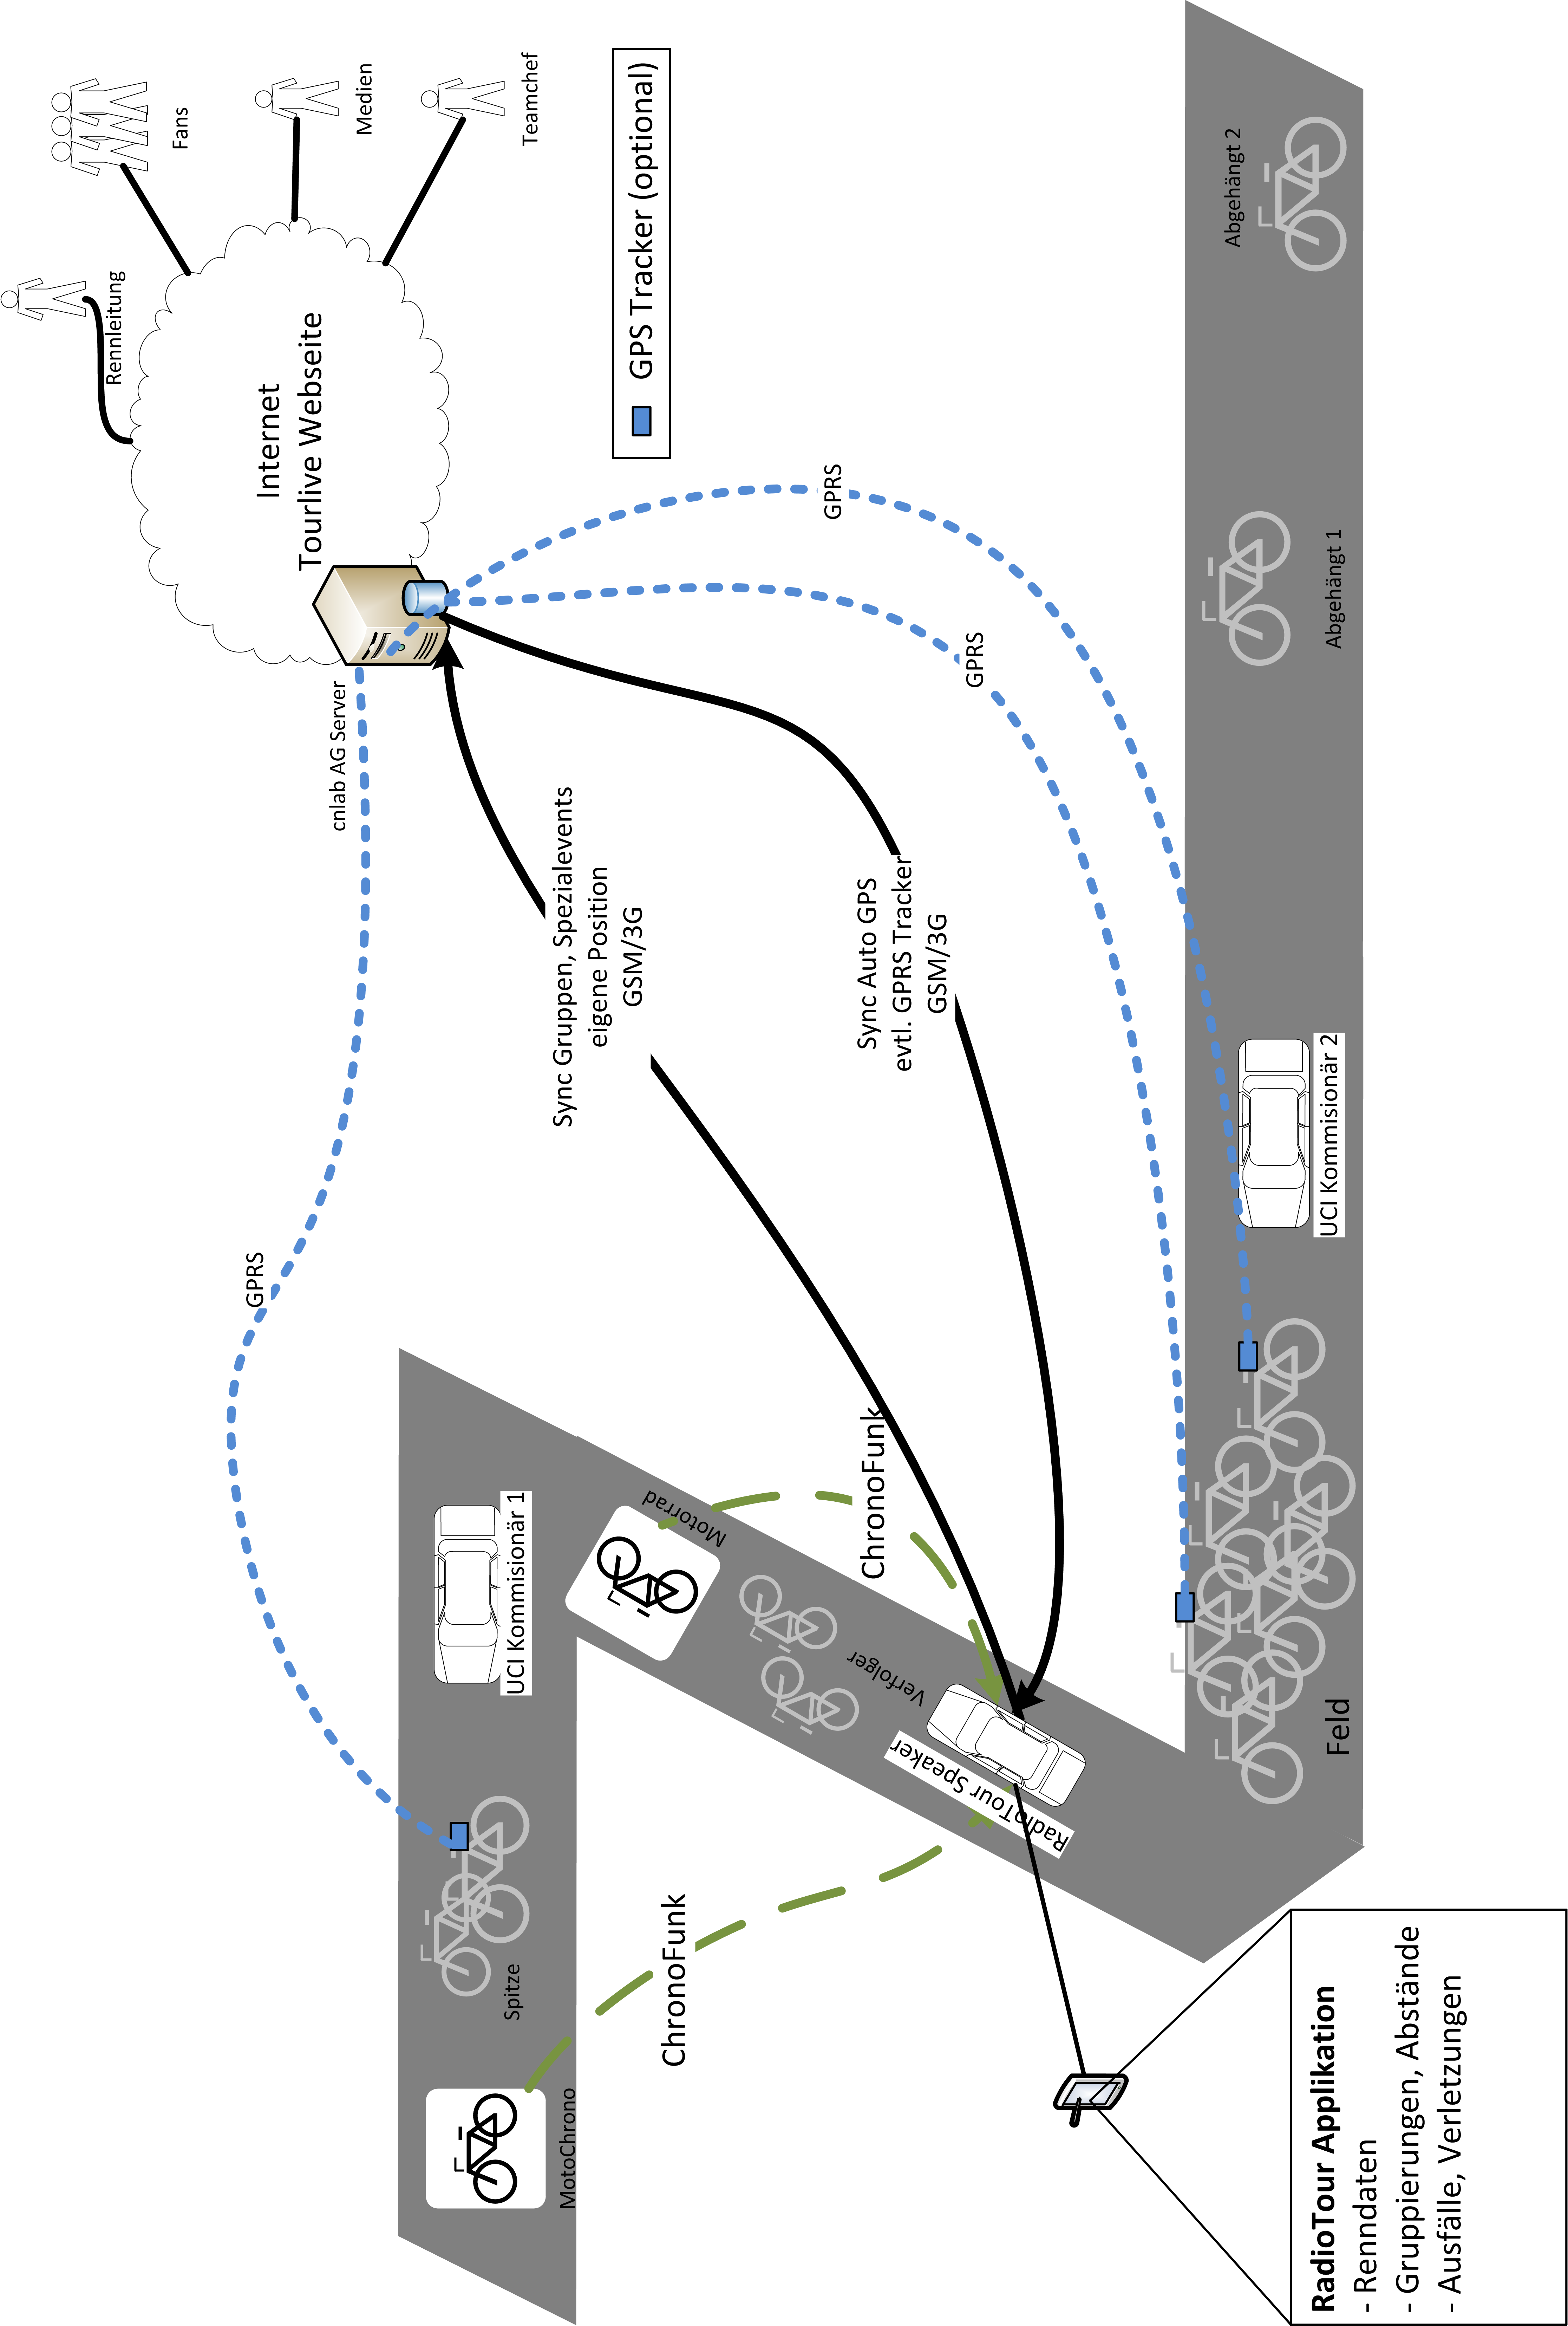
\includegraphics[scale=0.8]{07anhang/images/bigpicture.png}
\caption{Das BigPicture in voller Grösse}
\end{figure}

\section{Projektmanagement}

\section{Software Dokumente}

\section{Kriterienkatalog}
\label{ref_kriterien}
Hier sind die Kriterien

\section{Kaufempfehlung}
\label{ref_kaufempfehlung}

\section{UseCases der bisherigen Applikation}
\label{ref:usecases}
Im unten stehenden UseCase Diagramm (Abbildung \ref{fig:usecasediagram}) sind die primären UseCases aufgeführt. Nur der RadioTour Speaker erfasst Daten in dieser Applikation und ist daher der einzige Aktor. Das System wird durch die RadioTour Applikation abgebildet. Zur besseren Darstellung wurden einzelne UseCases vereinfacht oder zusammen gefasst.
\begin{figure}[h1]
  \caption{UseCase Diagramm}
  \label{fig:usecasediagram}
  \begin{center}
    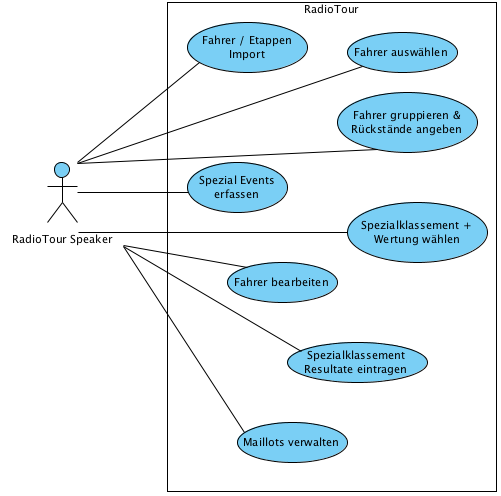
\includegraphics[scale=0.6]{05bericht/images/usecasediagram.png}
  \end{center}
\end{figure}

\begin{itemize}
\item \textbf{Fahrer auswählen}\\
Dem RadioTour Speaker muss es möglich sein, einen oder mehrere Fahrer schnell auszuwählen. Die Fahrer werden im Auswahldialog bevorzugt durch ihre Startnummern dargestellt. An der Tour de Suisse besteht ein Team – nach Aussage von P. Heinzmann – aus 8 Fahrern. Um eine möglichst gute Übersicht zu gewährleisten werden die Fahrer jeweils Zeilenweise in deren Teams gruppiert. Ausgewählte Fahrer werden farblich hervorgehoben. Die Nummern der Fahrer, welche bereits Gruppen zugewiesen wurden, werden in Klammern dargestellt. Die Nummern ausgeschiedener Fahrer werden gestrichen dargestellt.

\begin{figure}[h!]
  \caption{Die Fahrerauswahlliste zur Gruppierung in der bisherigen Web Applikation}
  \begin{center}
    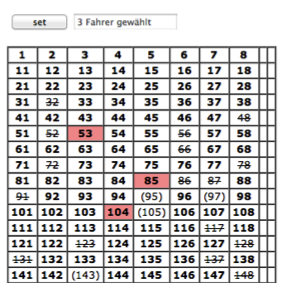
\includegraphics{05bericht/images/uc01_fahrerliste.png}
  \end{center}
\end{figure}

\item \textbf{Fahrer gruppieren}\\
Dem RadioTour Speaker muss es möglich sein, die ausgewählten Fahrer in Gruppen zu organisieren. So kann er die ihm gemeldeten Rennsituationen mit Ausreissern, Verfolgern, Feld und abgehängten darstellen.

\begin{figure}[H]
  \caption{Gruppierung in der bisherigen Web Applikation}
  \begin{center}
    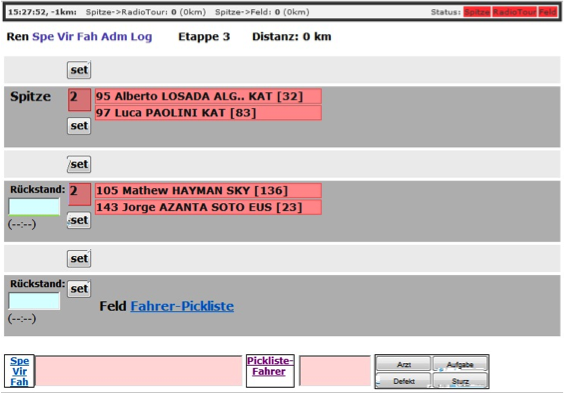
\includegraphics{05bericht/images/uc02_gruppen.png}
  \end{center}
\end{figure}

\item \textbf{Rückstände angeben}\\
Dem RadioTour Speaker muss es möglich sein, für die Gruppen (siehe oben) ihre jeweiligen Zeitabstände relativ zur Spitze einzugeben. Falls vorhanden, sollen auch die mit dem TourLive GPS-System erfassten Zeitabstände Spitze-Feld eingeblendet werden.

\item \textbf{Spezial Events erfassen}\\
Dem RadioTour Speaker muss es möglich sein, für ausgewählte Fahrer Spezialereignisse festzulegen. Dies sind beispielsweise Arztbesuch, Aufgabe, Defekt oder einen Sturz.
\begin{figure}[H]
  \caption{Die Spezialklassemente und Wertungen in der bisherigen Web Applikation}
  \begin{center}
    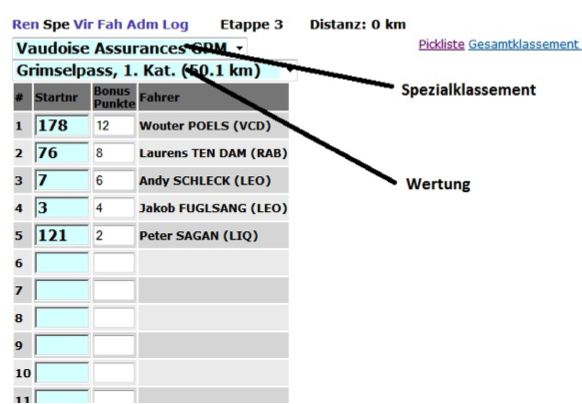
\includegraphics{05bericht/images/uc03_spezial.png}
  \end{center}
\end{figure}


\item \textbf{Spezialklassement und Wertung wählen}\\
Bei Mehretappenrennen werden typisch neben dem Gesamtklassement (schnellster Fahrer) mehrere Spezialklassemente (z.B. Bergpreis-, Sprintwertung, Punkteklassement) gewertet. Innerhalb der Etappen gibt es jeweils mehrere Stellen (Wertungen), an denen für die Spezialklassemente Punkte vergeben werden. Dem RadioTour Speaker muss es möglich sein, die gewünschte Wertung zu einem der vorher erfassten Spezialklassemente auszuwählen.

\item \textbf{Spezialklassement Resultate eintragen}\\
Dem RadioTour Speaker muss es möglich sein, für eine Wertung welche er ausgewählt hat (siehe UC oben), die Ränge zur Wertung mit Fahrernummern zu verbinden, wodurch das Klassement generiert wird.

\item \textbf{Klassement anzeigen}\\
Das durch die eingetragene Wertung erstellte Klassement muss vom RadioTour Speaker abgerufen werden können. Dort sollen alle Fahrer angezeigt werden, welche einen Punkterang in diesem Spezialklassement erreichten.

\item \textbf{Virtuelles Klassement}\\
Dem RadioTour Speaker muss es möglich sein, ein aktuelles Klassement der Tour abzurufen und dieses nach bestimmten Kriterien zu sortieren. Die zurzeit möglichen Sortierkriterien sind:
\begin{itemize}
\item[-]Gruppen (zur Zeit des Aufrufs, nicht offiziell)
\item[-]Virtueller Rückstand (zur Zeit des Aufrufs, nicht offiziell)
\item[-]Zeitboni (zur Zeit des Aufrufs, nicht offiziell)
\item[-]Offizielle Zeit (zum Etappenende des Vortages, offiziell)
\item[-]Offizieller Rückstand (zum Etappenende des Vortages, offiziell)
\end{itemize}

\begin{figure}[h!]
  \caption{Virtuelles Klassement in der bisherigen Applikation}

  \begin{center}
    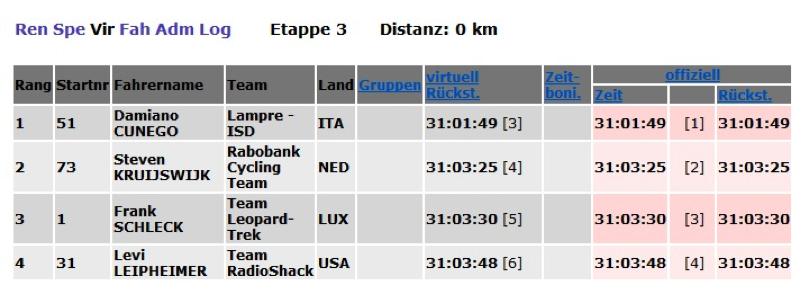
\includegraphics{05bericht/images/uc05_virtuell.png}
  \end{center}
\end{figure}

\item \textbf{Fahrerliste anschauen}\\
Dem RadioTour Speaker muss es möglich sein, die aktuelle Fahrerliste anzuschauen. Die Fahrerliste ist nach Startnummer aufsteigend sortiert. (Die Startnummern werden in Mehretappenrennen so vergeben, dass die Fahrer eines Teams aufeinanderfolgende Startnummern erhalten.)

\begin{figure}[h!]
  \caption{Die Fahrerliste mit den Informationen zum Status der Fahrer}
  \begin{center}
    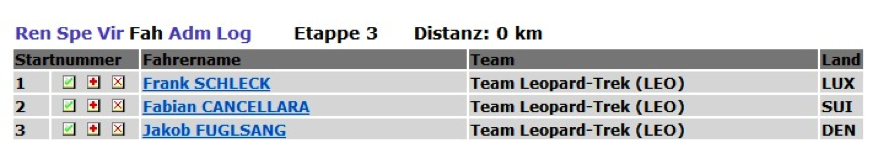
\includegraphics{05bericht/images/uc06_fahrerliste.png}
  \end{center}
\end{figure}

\item \textbf{Fahrer de- bzw. aktivieren}\\
Dem RadioTour Speaker muss es möglich sein, einzelne Fahrer zu deaktivieren bzw. wieder zu aktivieren. Der Grund der Deaktivierung soll auch später noch nachvollziehbar sein. Es soll möglich sein, den Grund für die Deaktivierung anzugeben (z.B. ausgeschieden, nicht gestartet, andere). 
Eine so vorgenommene Deaktivierung eines Fahrers muss durch den RadioTour Speaker Rückgängig gemacht werden können.

\item \textbf{Fahrerdetails bearbeiten}\\
Dem RadioTour Speaker muss es möglich sein, einen Fahrer aus der Fahrerliste auszuwählen um seine Details anzuschauen und auch zu bearbeiten. 

\item \textbf{Statistik}\\
Dem RadioTour Speaker muss es möglich sein, in seinem Admin-Bereich eine kurze und prägnante textbasierte Statistik zu erhalten, bei welcher er auf einen Blick sieht wie viele Fahrer in der Datenbank sind und welche davon aktiv sind. Darüber hinaus die Anzahl Gruppen, Spezialklassemente, Wertungen und Vergebene Punkte.

\item \textbf{Import Fahrerliste}\\
Nach jedem Renntag ( = Etappe), wird in die RadioTour Applikation eine neue Fahrerliste mit den aktuellen offiziellen Zeiten importiert. Die Herausforderung besteht darin, dass das Format dieser Fahrerlisten im vornherein nicht bekannt ist. Deshalb muss es dem RadioTour Speaker möglich sein, den Importmodus noch dynamisch anzupassen. Derzeit sind für den Import der Daten verschiedene Importverfahren implementiert wie im Screenshot ersichtlich ist.

\item \textbf{Import Spezialklassemente}\\
Dem RadioTour Speaker muss es möglich sein, Spezialklassemente zu importieren. Diese Importe werden vor der Tour de Suisse getätigt weshalb ein dynamischer Import hier nicht zwingend notwendig ist.

\item \textbf{Speicherung Maillots}\\
Dem RadioTour Speaker muss es möglich sein, die Belegung der 4 verschiedenen Maillots anzugeben und zu sichern. Folgende Maillots gibt es:

\begin{center}
  \begin{tabular}{ l | l  }
    \hline
    Name & Farbe \\ \hline
    \hline
    Bergpreis & Rot-Weiss \\ \hline
    Gesamtklassement & Gelb \\ \hline
    Neo-Profi & Weiss \\ \hline
    Punkte & Grün\\

    \hline
  \end{tabular}
\end{center}


\item \textbf{Daten exportieren}\\
Dem RadioTour Speaker muss es möglich sein, die Spezialklassemente, Wertungen, Fahrer nicht nur zu erfassen, importieren und bearbeiten, sondern auch als *.csv zu exportieren. Dabei werden einfach alle mit dem gewünschten Export assoziierten Infos in das exportierte *.csv geschrieben.

\end{itemize}

